\documentclass[bachelor,substylefile = VolSU.rtx]{disser}

\usepackage[
  a4paper, mag=1000,
  left=3.0cm, right=1cm, top=2cm, bottom=2cm, headsep=0.7cm, footskip=1cm
]{geometry}

\usepackage[T2A]{fontenc}
\usepackage[utf8]{inputenc}
\usepackage[english, russian]{babel}


\usepackage{amsmath, amssymb, amsfonts}
\usepackage{graphicx, epsfig}
\usepackage{enumitem}
\usepackage{listings}
\lstset{
    language=Python,
    breaklines=true,
    tabsize=2,
    numberbychapter=false,
    columns=fixed,
    showstringspaces=false,
    showtabs=false,
    keepspaces,
    extendedchars=\true
}


\usepackage{caption}
\usepackage{longtable}
\usepackage{float}

\usepackage{color}
\usepackage[colorlinks=false,linkcolor=blue,breaklinks]{hyperref}

\usepackage[citestyle=gost-numeric,style=gost-numeric,maxnames=100,natbib=true,urldate=long, sorting=none]{biblatex}
%\bibliographystyle{ugost2008ns.bst} 
\pagestyle{footcenter}
\chapterpagestyle{footcenter}

%для борьбы с переполнениями за счет разреженных слов в абзаце
\emergencystretch=5em


\graphicspath{{fig/}}
\addbibresource{Bib.bib}

\begin{document}

\renewcommand{\labelenumii}{\arabic{enumi}.\arabic{enumii}}
\renewcommand{\labelenumiii}{\arabic{enumi}.\arabic{enumii}.\arabic{enumiii}}
\renewcommand{\labelenumiv}{\arabic{enumi}.\arabic{enumii}.\arabic{enumiii}.\arabic{enumiv}}

\institution{Волгоградский государственный университет \\
Институт математики и информационных технологий \\
Кафедра информационных систем и компьютерного моделирования}

% Название практики и семестр
\title{Отчет по производственной практике, преддипломной практике}
\semester{восьмой семестр}
\topic{Кроссплатформенная информационная система для обмена сообщениями}

\apname{А. В. Хоперсков}
% Автор
\author{Мостовой Максим Сергеевич}
\authorshort{М. С. Мостовой}
% Группа
\group{ИСТб-191}
\coursenum{09.03.02}
\course{Информационные системы и технологии}

% Руководитель практики
\supervisor       {Н. С. Полусмакова}
\supervisorstatus {к.э.н., доцент каф. ИСКМ}
% Организатор практики
\organizer        {Р. В. Щёлоков}
\organizerstatus  {к.ф.-м.н., доцент каф. ИСКМ}
% Научный консультант
\consultant       {Д. Н. Фокин}
\consultantstatus {ассистент каф. ИСКМ}
%
\city{Волгоград}
\date{\number\year}

\maketitle

\renewcommand\contentsname{Содержание}
\tableofcontents

\intro
 Одними из широко применяемых динамических систем яввляются системы с перемееной структурой~\cite{578556}. Данной системе характерно изменение своего поведения в зависимости от изменения многих факторов, которые воздействуют на неё, как в ней самой так и из вне. Моделирование систем с переменной структурой часто применяетсмя в таких областях как автоматическое управление~\cite{5498611}, робототехника~\cite{1}, автомобильной промышленности~\cite{2}, электроника~\cite{3}  и многое другое. Кроме того, с развитием технологий и появлением новых приложений, таких как автономные системы, робототехника и многие другие, моделирование систем с переменной структурой остается актуальной темой и требует дальнейших исследований и разработок.

 Целью работы является изучение различных систем с переменной структурой и разработка программы  на примере исследования какой-либо известной математической модели.

 В ходе выполнения производственной практики были выполнены следующие задачи:
\begin{enumerate}
\item[—] анализ необходимой литературы по предметной области;
\item[—] изучение особенностей систем с переменной структурой;
\item[—] изучение особенностей перевернутого маятника и нелинейнного регулятора;
\item[—] реализация программы для создания математической модели в среде визуального программирования;
\item[—] написание отчета по производственной практике.
\end{enumerate}

Отчет по производственной практике состоит из введения, трёх глав, заключения
и приложения.

Во введении обоснована актуальность выбранной темы, сформулированы цели и задачи изучения моделирования систем с переменной структурой.

В первой главе рассмотрено и описано понятие понятие динамических систем и их классификация, которая способствуют для понимания систем с переменной структурой. Описаны нелинейные элементы и характеристики.

Во второй главе рассмотрена и описана система с переменной структурой.

В третьей главе представлена реализация создания математической модели для перевернутого маятника и нелинейного регулятора в среде визуального программирования.

В заключении подведены основные итоги проделанной работы, а так же
сформулированы основные выводы.

В приложении предоставлен исходный код разработанной программы.


\chapter{Понятие цифровых моделей местности и их классификация}

Цифровая модель местности (ЦММ) – это множество элементов, являющиеся топографо-геодезической информацией о местности.
ЦММ включает в себя: 

\begin{enumerate} 
  \item[1)] метрическую информацию о геодезических пространственных координатах характерных точек рельефа и ситуации;
  
  \item[2)] синтаксическую информацию, используемую для описания связей между точками границ зданий, лесов, водоемов, дорог, водораздельных и водосливных линии и т.п.;
  
  \item[3)] семантическую информацию, характеризующую свойства объектов, а именно технические параметры инженерных сооружений, геологические характеристики грунтов, данные о деревьях в лесных массивах и т.п.;
  
  \item[4)] структурную информацию, описывающую связи между различными объектами, отношения объектов к какому-либо множеству, например, раздельные пункты железнодорожной линии, здания и сооружения населенного пункта, строения и конструкции производств и т.п.;
  
  \item[5)] общую информацию, это может быть название участка, система координат и высот, номенклатура \cite{19,10}.
  
\end{enumerate} 


ЦММ характеризует ситуацию и рельеф местности. Она состоит из цифровой модели рельефа (ЦМР) и цифровой модели контуров (ЦМК). Кроме этого ЦММ может дополняться моделью специального инженерного назначения (ЦМИН) \cite{11}.

\section{Цифровые модели рельефа}

Цифровая модель рельефа представляет собой поверхность местности, которая не включает в себя объекты, находящиеся на поверхности, которая создается на основе данных о высоте. Поверхность местности может быть представлена как трехмерная (3D) или двумерная (2D) \cite {1, 23}.

Источники для исходных данных для построения ЦМР очень разнообразны: 

\begin{enumerate} 
  \item[1)] радарная топографическая съемка местности;
  \item[2)] методы кинематической глобальной навигационной спутниковой системы;
  \item[3)] данные дистанционного зондирования Земли;
  \item[4)] материалы полевых съемок;
  \item[5)] методы определения структуры по движению;
  \item[6)] интерполяция цифровых контурных карт или данных из прямых съемок поверхности земли и другие \cite{2, 17}.
\end{enumerate} 

С помощью ЦМР можно автоматически извлечь морфометрические данные, такие как уклоны и изломы, аспект уклона, альтиметрические пояса, шероховатость или зернистость поверхности, а также параметры, касающиеся гидрографических сетей. Также при использовании ЦМР можно решить задачи связанные с оценкой форм склонов, через кривизну их поперечного сечения, проведением интерполяции по значениям высот, проведением трехмерной визуализации рельефа, проведением оценки видимости или невидимости  с определенной точки обзора и многие другие \cite{15,13}.

Существуют определенные требования, которым цифровая модель рельефа должна соответствовать:

\begin{enumerate} 
  \item[1)] модель должна содержать в себе доступную информацию, которую получают в результате наблюдений;
  \item[2)] параметры, которые присущи модели, должны иметь однозначный физический смысл и возможность прямого измерения;
  \item[3)] систематизация значений параметров позволит использовать их при моделировании стока в малоизученных бассейнах \cite{3,21}.
\end{enumerate} 

Также модель рельефа может быть представленна как матрица высот или матрица качеств.

\subsection{Матрицы высот рельефа местности}

Матрица высот может быть построена по тем данным объектов карты рельефа местности, которые имеют абсолютную высоту или 3D-метрику. В задачах анализа рельефа, которых касаются построения профилей и зон видимости, а также в задачах вычисления площади или длины объекта с учетом рельефа такая матрица высот может использоваться в качестве основы. Также в задачах моделирования зон затопления, формирования объемной карты местности, определения направления склонов и других \cite{4,12}.

\begin{figure}[h!]
    \center
    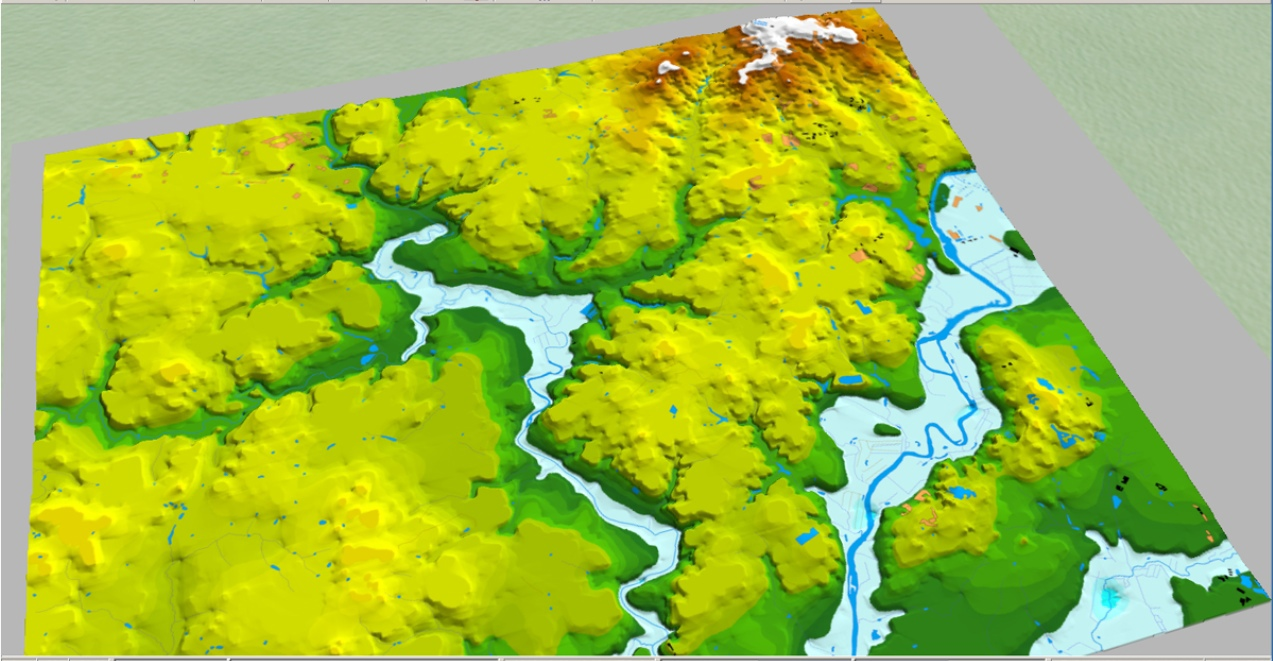
\includegraphics[scale=0.3]{images/112.jpg}
    \caption{Пример матрицы высот}
    \label{fig:1}
\end{figure}

Для формирования трехмерной метрики определенных объектов, содержащихся на карте, или для получения отмывки рельефа в виде растрового изображения, оценки и анализа статистики поверхности указанного участка местности, а также для создания автоматического построения изолиний -- используют матрицу высот рельефа \cite{5,14}. Пример матрицы высот изображен на рисунке
\ref{fig:1}.

\subsection{Использование матриц качеств для характеристик поверхности}

Обычно матрицу качеств представляют в виде поверхности значений определенной моделируемой характеристики. Для построения матрицы качеств могут использоваться значения смысловой характеристики объектов, содержащиеся на векторной карте или в выбранных полях таблицы базы данных \cite{6, 7}. 

Данные, которые может содержать матрица качеств очень различны. Это может быть, как тип растительности или землевладения, плотность застройки, так и качественные характеристики почвы, глубина залегания грунтовых вод, концентрация выхлопных газов и т.д.

Модель поверхности, которая представлена матрицей качеств, можно изменить, выполняя определенные операции (арифметические и логические) над её элементами. Используя матрицу качеств можно осуществить анализ определенной моделируемой характеристики с помощью поиска областей, значения характеристики в которых удовлетворяют набору заданных условий. Результаты такого анализа могут сохранятся в двух видах -- растрового изображения или матрицы качеств \cite{8,16}. Пример матрицы качеств изображен на рисунке \ref{fig:2}.

\begin{figure}[h!]
    \center
    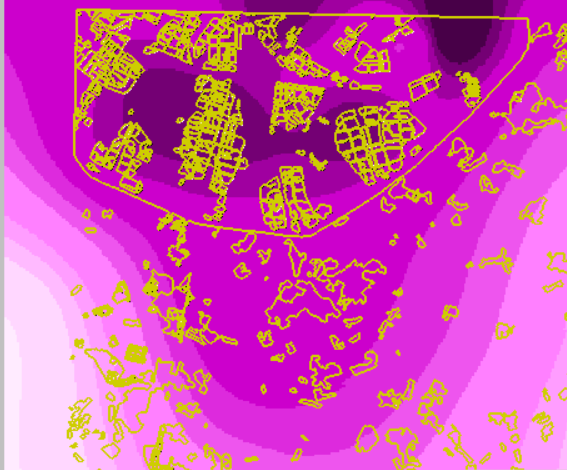
\includegraphics[scale=0.7]{images/111.png}
    \caption{Пример матрицы качеств концентрации выхлопных газов}
    \label{fig:2}
\end{figure}

\subsection{Классификация цифровых моделей рельефа}
Классифицировать ЦМР можно по нескольким признакам, например по характеру нахождения объектов: регулярные и нерегулярные.

В регулярных ЦМР заметно, что точки моделирующие поверхность земли находятся в пересечении узлов сетки, которую проецируют на местность. В подобной сетке форма ячеек может являться различными геометрическими объектами: прямоугольники, квадраты, равносторонние треугольники (рисунок ~\ref{fig:3}).

\begin{figure}[h!]
    \center
    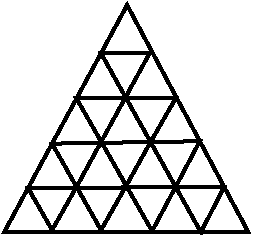
\includegraphics[scale=2]{images/regular.png}
    \caption{Пример регулярной сетки}
    \label{fig:3}
\end{figure}

Такая ЦМР наиболее проста, так как легче провести ее построение, особенно если в районе, в котором строится ЦМР, проводились геодезические работы \cite{9,20}. 

Эффективность, достигаемая в условиях однородной местности или городской застройки, является достойным преимуществом регулярной ЦМР.

Основными минусами регулярной ЦМР являются:  

\begin{enumerate} 
  \item[1)] ключевые точки рельефа, такие как вершины, впадины, глубины, границы оврагов и т.п., не всегда  совпадают с узлами сетки;
  \item[2)] регулярные ЦМР требуют много трудозатрат при разбиении узловых точек на местности и определении значений высоты в каждой из них;
  \item[3)] при резко меняющемся рельефе, особенно если размеры ячеек очень большие, значительная часть информации может не отразиться в ЦМР (например овраги);
  \item[4)] при слишком маленьких размерах ячеек на достаточно однородной части рельефа, может случиться переизбыток точек, будет занят довольно большой объем памяти и потребуются лишние затраты времени и труда на ввод отметок высоты в узлах сетки \cite{19,22}.
\end{enumerate} 

Регулярные модели нашли применение при проектировани аэродромов, городских улиц, при вертикальной планировке, то есть тогда, когда требуется повышенная детальность исходной информации. 

Также существуют нерегулярные ЦМР, в которых точки размещаются в произвольном порядке, но при этом с заданной частотой и плотностью. Чем сложнее рельеф на местности, тем гуще должна быть построенная сетка (рисунок~\ref{fig:4}). Такая ЦМР позволяет ввести все ключевые точки рельефа~\cite{10}.

Одним из видов нерегулярной сетки является образующаяся при сканировании различных топографических материалов сетка.

У ЦМР, построенной на основе такой сетки, также имеется недостаток~--~для каждой точки необходимо вводить ее номер, координаты $x$, $y$ и отметки высот $h$.

После того как ключевые точки рельефа нерегулярной сетки будут отображены на карту, по данным этих точек будет строиться модель поверхности одним из существующих методов \cite{11,18}. 

\begin{figure}[h!]
    \center
    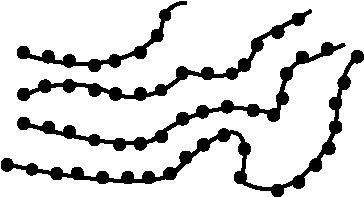
\includegraphics[scale=2.5]{images/unregular.png}
    \caption{Пример нерегулярной сетки}
    \label{fig:4}
\end{figure}

\section{Цифровая модель контуров}

Цифровая модель контуров, также называемая цифровой моделью ситуации, состоит из совокупности точечных, линейных и площадных топографических объектов, с заданными координатами принадлежащих им точек и семантической информацией в виде списка характеристик, значения которых можно изменять. 

Семантика ЦМК имеет влияние на представление элемента в разных видах, таких как план, профиль, сечение, 3D-вид. Атрибуты должны определять как качественные параметры, например, треугольная труба или шестиугольная в сечении, тропическое растение или лиственное, так и количественные параметры объектов, например, длина, площадь. Связи таких атрибутов между собой определяют не только вид, но и поведение элемента в разных ситуациях и проекциях \cite{18,20}.

На рисунке \ref{fig:5} представлена цифровая модель контуров. Точки контуров (углы зданий, углы поворота линейных объектов и т.д.) определяют значения координат $X$ и $Y$ без значения высоты $H$. Также указана взаимосвязь точек контура, например, группа точек (1,2,3,4) определяет сплошной контур жилого дома, а группа точек (15,16,17,18) определяет контур дороги.

\begin{figure}[h!]
    \center
    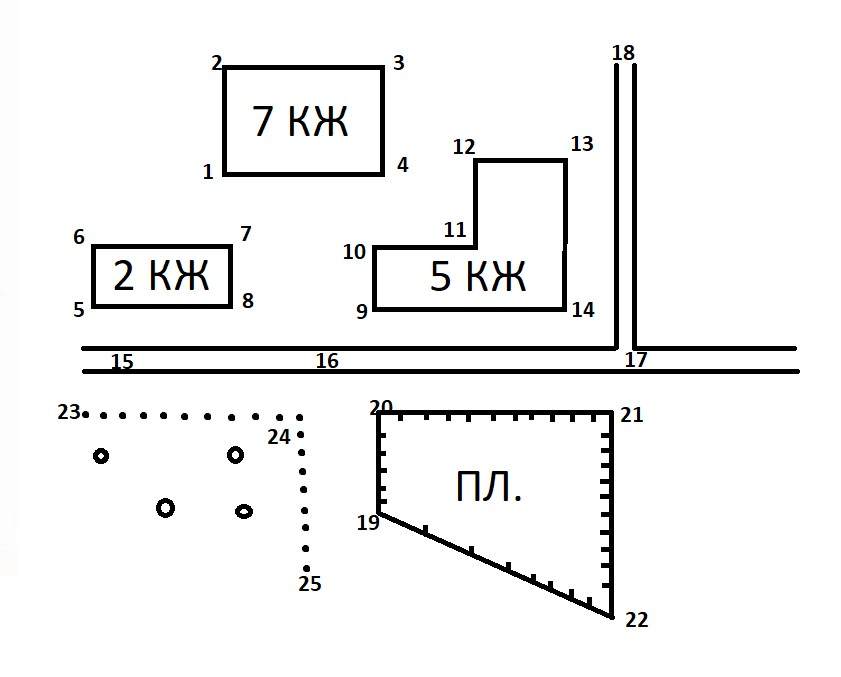
\includegraphics[scale=0.52]{images/1717.jpg}
    \caption{Пример цифровой модели контуров}
    \label{fig:5}
\end{figure}

\section{Цифровые модели специального инженерного назначения}

Цифровые модели специального инженерного назначения широко используются в виде результатов инженерно-геодезических изысканий. Проектировщику нужно принимать определенные решения, которые касаются решений по проекту, пользуясь в качестве исходных данных физическим состоянием определенной местности. Это требует, кроме соблюдения норм инженерно-геодезических изысканий, таких как состав, полнота данных, точность, еще и таких условий как: 

\begin{enumerate} 
  \item[1)] соответствие ЦМР её топографической реальности;
  \item[2)] пространственного представления в модели подземных и надземных коммуникаций;
  \item[3)] многослойности модели рельефа и ситуации с заданным распределением данных, необходимых проектировщику, по отдельно организованным слоям;
   \item[4)] информационной насыщенности объектов модели сведениями, необходимыми для принятия проектных решений и согласований \cite{22}.
\end{enumerate} 

\section{Классификация цифровых моделей местности}

ЦММ полностью соответствуют классификации карт по назначению, а именно топографические, контурные, геологические, кадастровые и др.

Цифровые модели местности делятся на четыре типа по способу размещения их исходной информации и правил ее обработки на электронно-вычислительной машине (ЭВМ). 

\begin{enumerate} 
  \item[1.] Регулярные, в которых опорные точки с известными координатами располагаются в узлах геометрических сеток различной формы (рисунок~\ref{fig:6}~а) регулярная сетка ЦММ). Такие используют для равнинной местности.
 
  \item[2.] Нерегулярные, в которых точки располагаются произвольно в пределах однородных по рельефу, геологии, гидрологии участков местности без какой-либо определенной системы, но с заданной густотой и плотностью (рисунок~\ref{fig:6}~б) нерегулярная сетка ЦММ).

  \item[3.] Структурные, в которых точки с известными координатами расставлены в вершинах переломов структурных (орографических) линий рельефа. Точки таких ЦММ могут распологаться на основных перегибах всех структурных линий: рисунок~\ref{fig:7}~(а)~--~ структурная сетка, точки которой располагаются вдоль скатов в местах изменения кривизны склонов, рисунок~\ref{fig:7}~(б)~--~ структурная сетка, точки которой расположены на основных перегибах, вдоль скатов по линии наибольшей крутизны в местах характерных переломов с указанием крутизны и направлений линий, рисунок~\ref{fig:7}~(в)~--~структурная сетка, точки которой расположены в местах изменения кривизны склонов. Структурные ЦММ используют для пересеченной местности.

   \item[4.] Статические -- основаны на определении координат точек, случайно и часто выбранных на местности~\cite{23}.
\end{enumerate} 

 \begin{figure}[h]
    \begin{minipage}[h]{0.5\linewidth}
    \center{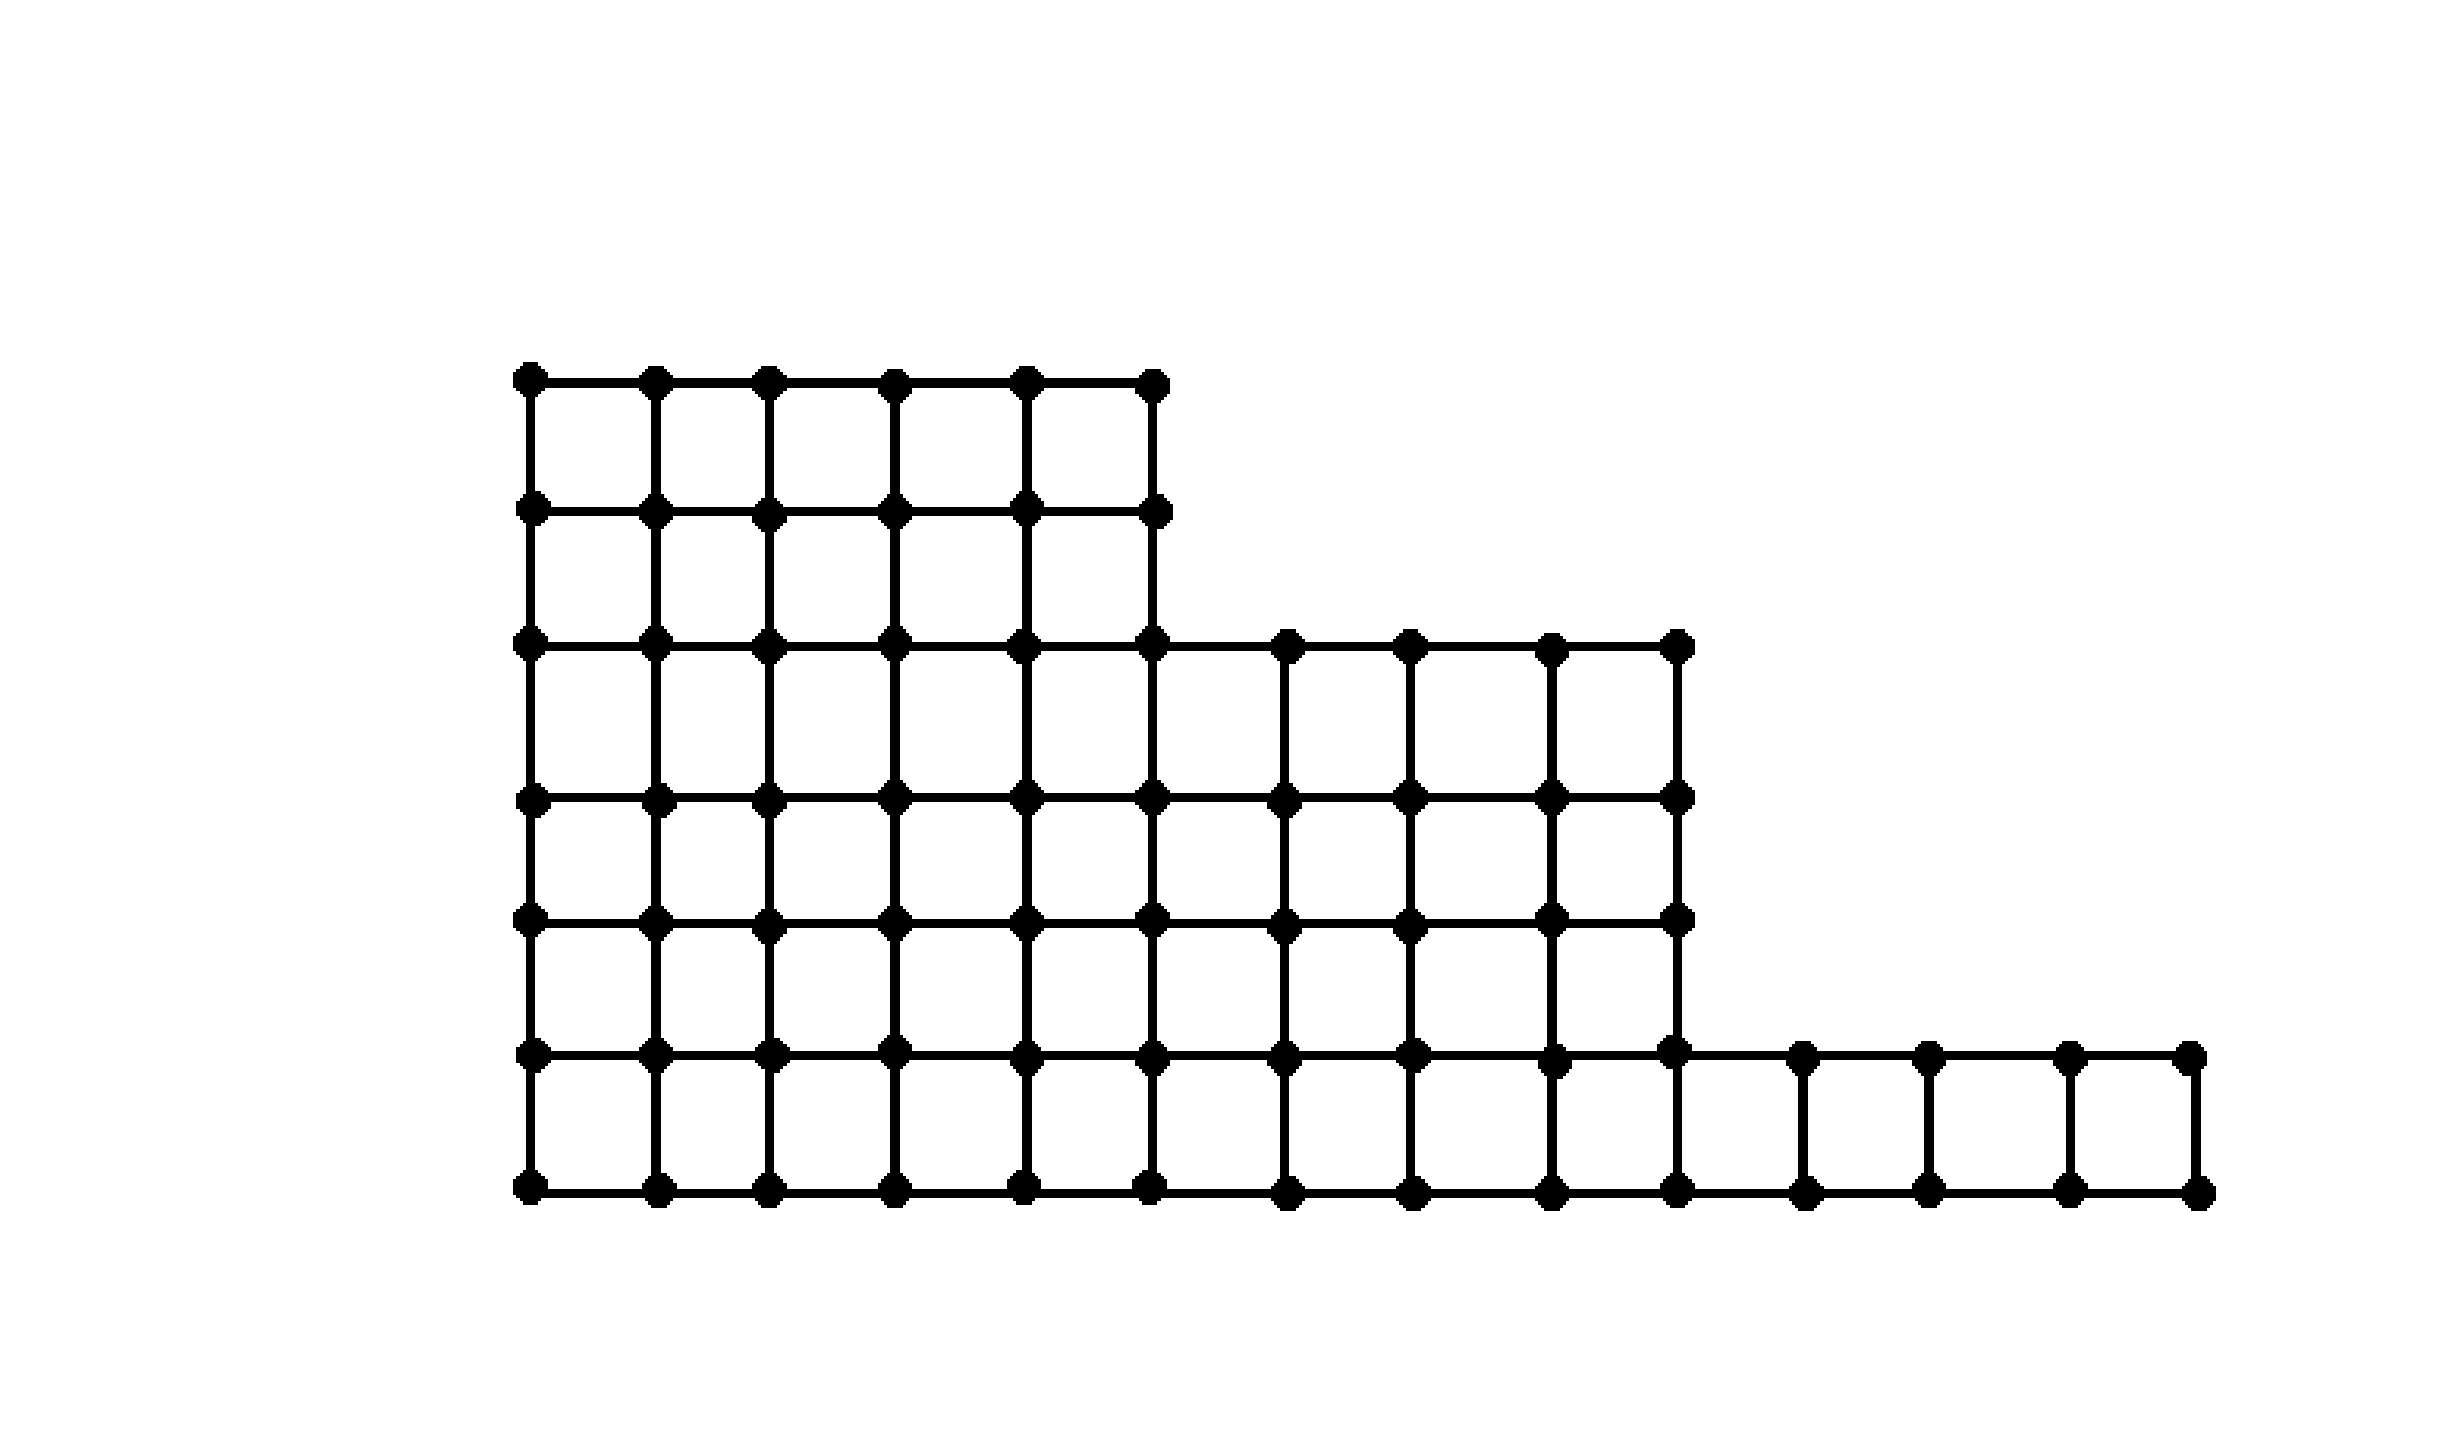
\includegraphics[width=1\linewidth]{images/11111.png} \\ а)}
    \end{minipage}
    \hfill
    \begin{minipage}[h]{0.5\linewidth}
    \center{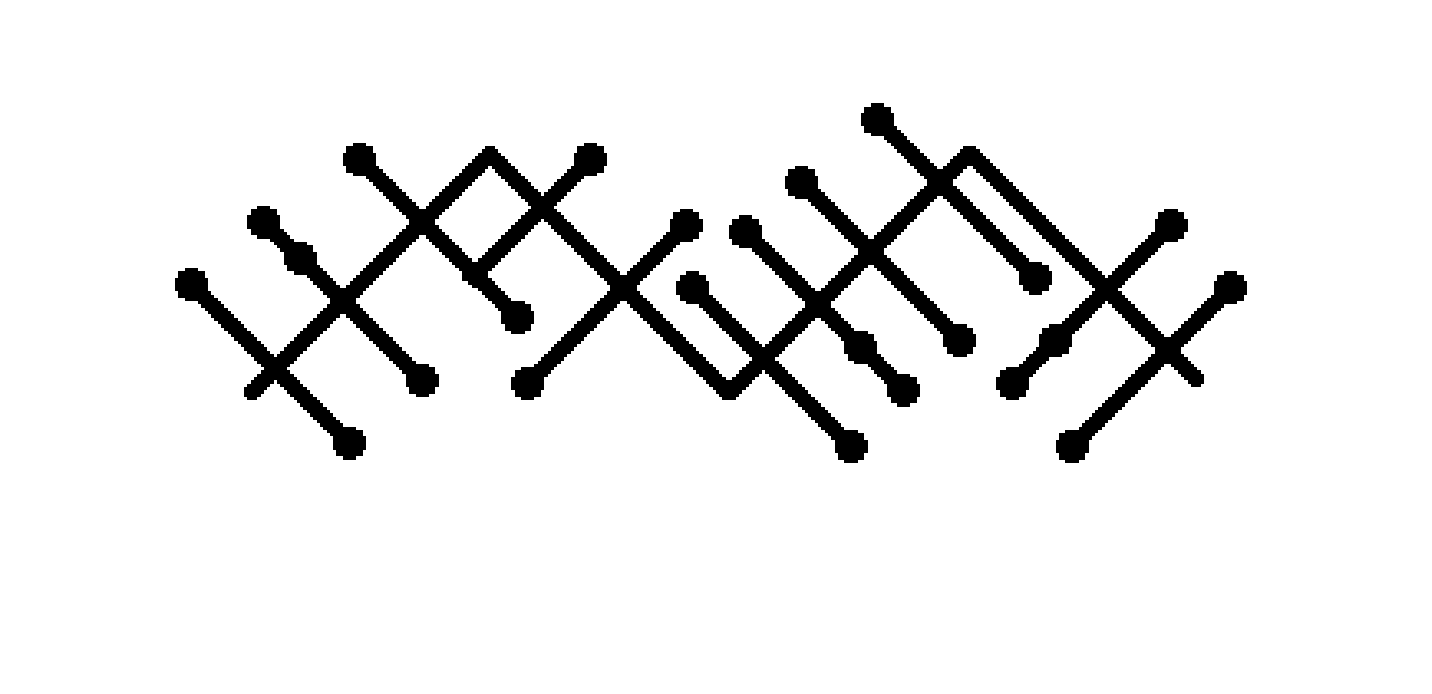
\includegraphics[width=1\linewidth]{images/161616.png} \\ б)}
    \end{minipage}
\caption{Пример регулярной и нерегулярной сетки ЦММ}
\label{fig:6}
\end{figure}
 
\begin{figure}[h]
    \begin{minipage}[h]{0.2\linewidth}
    \center{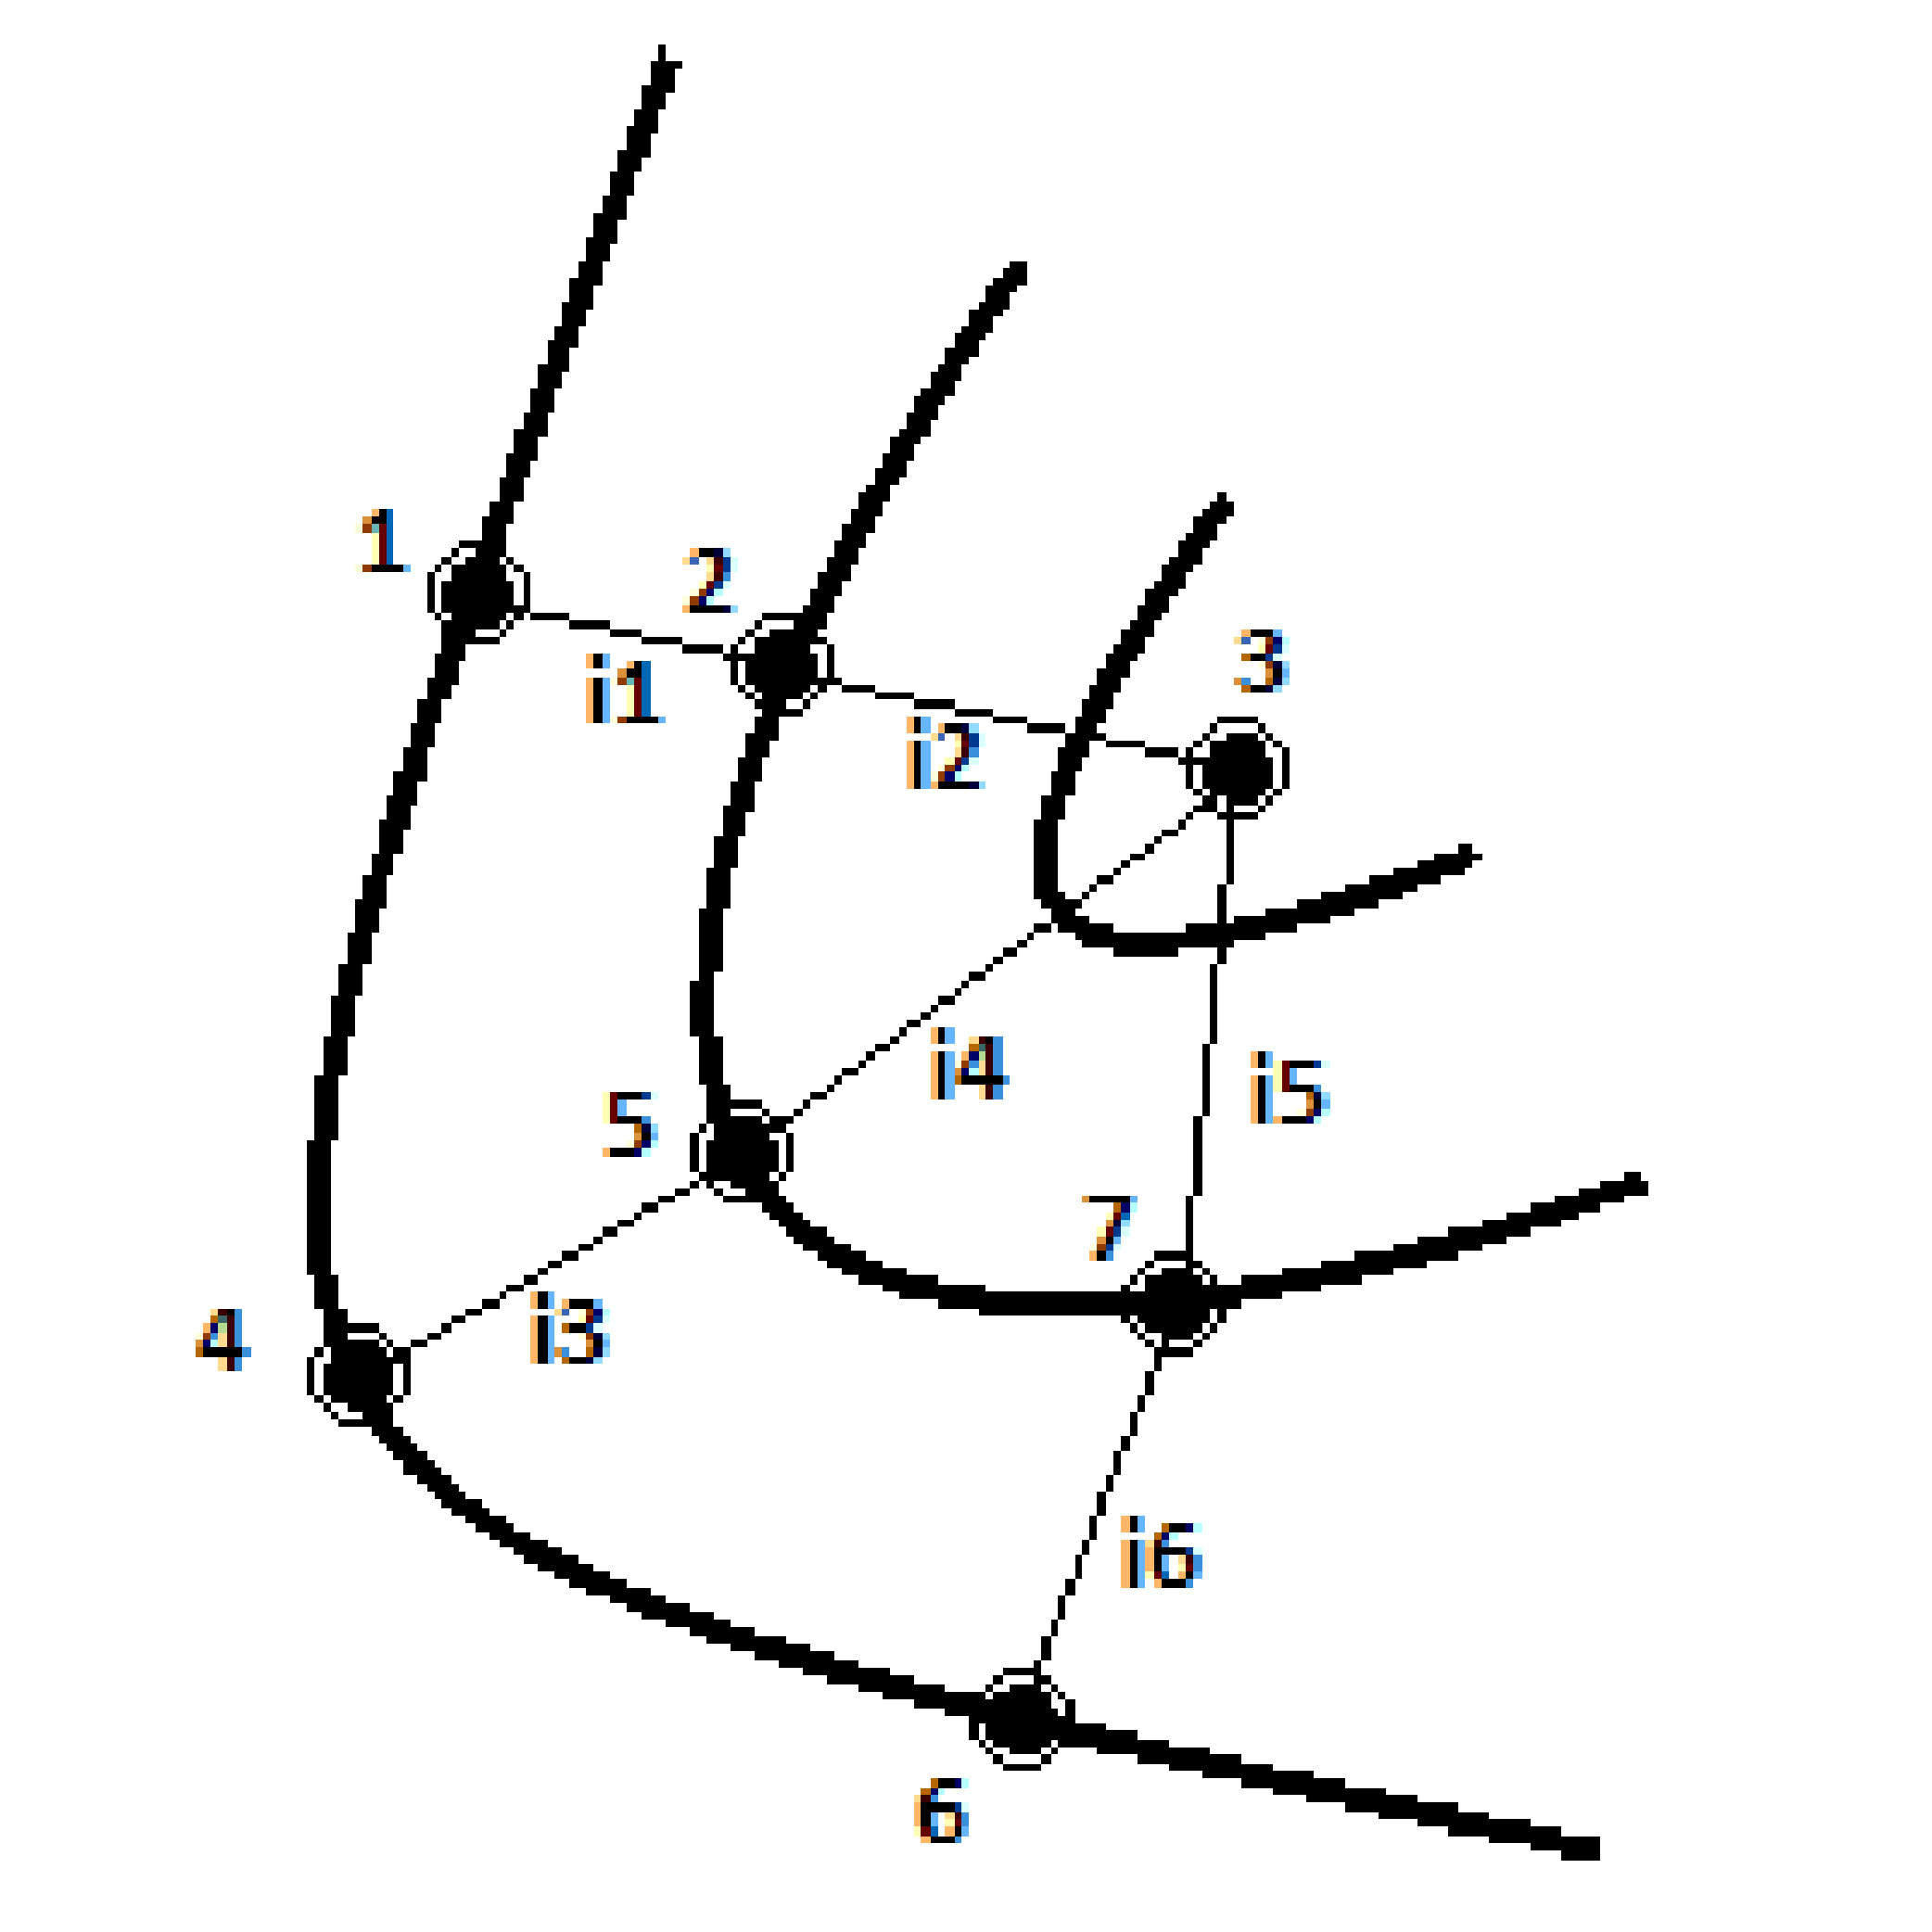
\includegraphics[width=1\linewidth]{images/151515.png} \\ а)}
    \end{minipage}
    \hfill
    \begin{minipage}[h]{0.2\linewidth}
    \center{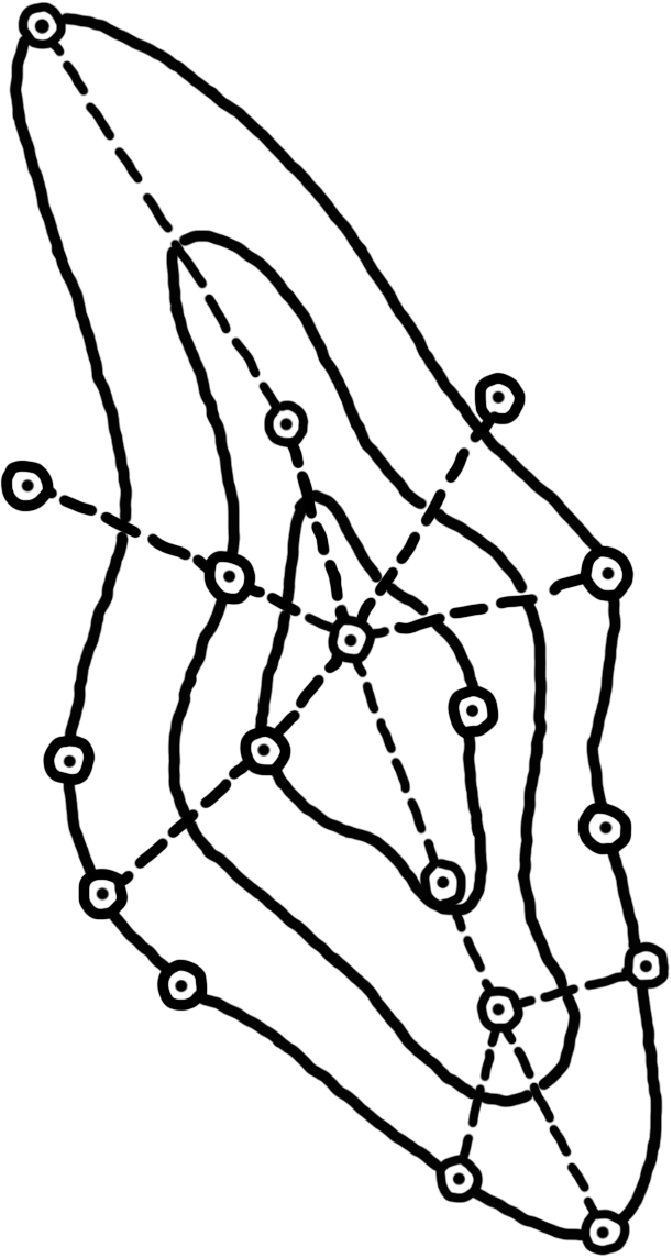
\includegraphics[width=0.8\linewidth]{images/888.png} \\ б)}
    \end{minipage}
    \hfill
    \begin{minipage}[h]{0.2\linewidth}
    \center{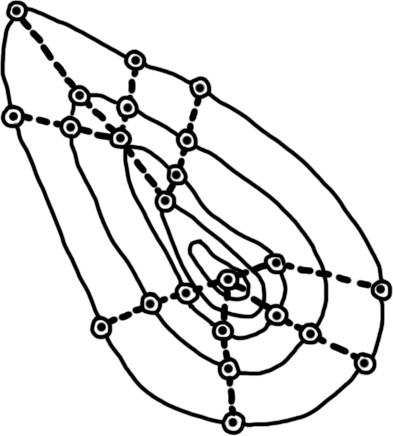
\includegraphics[width=0.8\linewidth]{images/7777.png} \\ в)}
    \end{minipage}
\caption{Примеры сеток структурной ЦММ}
\label{fig:7}
\end{figure}


\chapter{Проектирование информационной системы «Личный кабинет абитуриента»}

\section{Проектирование архитектуры веб-приложения}

Перед началом проектирования архитектуры веб-приложения, следует выбрать какой тип архитектуры использовать. Существует множество различных подходов проектирования архитектуры веб-приложений, самые популярные на текущий момент это микросервисная архитектура и монолитная архитектура, которая, как правило, представляет собой веб-приложение с 3-х уровневой архитектурой \cite{webapacrch}.

Монолитная архитектура является традиционным методом разработки веб-приложений. Монолитное приложение полностью замкнуто в контексте поведения. Во время работы оно может взаимодействовать с другими службами или хранилищами данных, однако основа его поведения реализуется в собственном процессе, а все приложение обычно развертывается как один элемент (рисунок \ref{fig:monolit}). Для горизонтального масштабирования такое приложение обычно целиком дублируется на нескольких серверах или виртуальных машинах \cite{monolith}. Как правило, такие приложения состоят из следующих слоев:

\begin{enumerate} 
  \item слой представления — содержит пользовательский интерфейс и отвечает за обеспечение хорошего пользовательского опыта;
  
  \item слой бизнес-логики — отделяет пользовательский интерфейс от вычислений, связанных с бизнесом;
  
  \item слой передачи данных — отвечает за взаимодействие с постоянными хранилищами, такими как базы данных, и прочую обработку информации, которая не связана с бизнесом.
\end{enumerate}

\begin{figure}[H]
\begin{center}
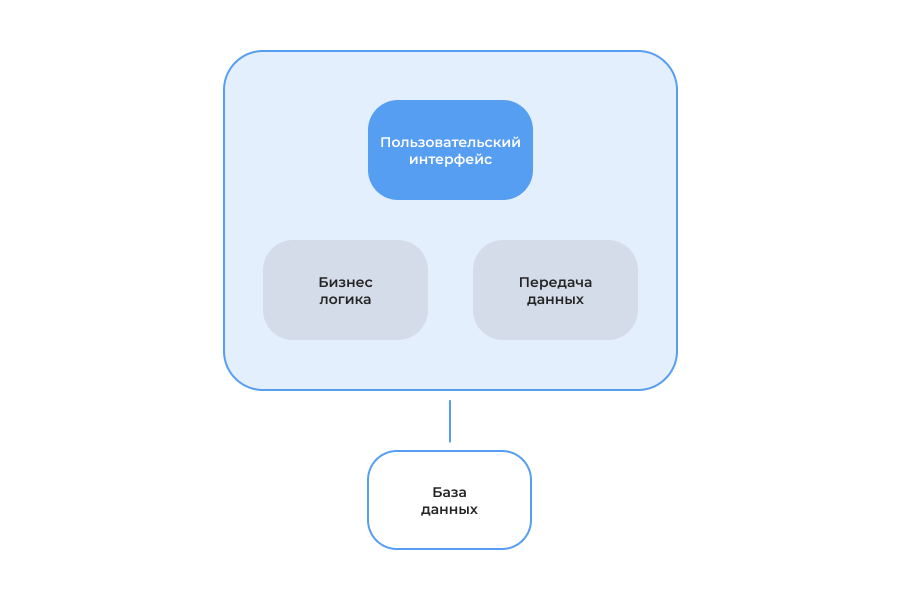
\includegraphics[width=0.9\hsize]{fig/monolit.png}\\[2mm]
\caption{Архитектура монолитного приложения из трех слоев}\label{fig:monolit}
\end{center}
\end{figure}

Преимущества монолитной архитектуры:

\begin{enumerate} 
  \item упрощенная разработка и развертывание — благодаря монолитному ядру все изменения и обновления развертываются вместе;
  
  \item быстрая связь между программными компонентами благодаря общему коду и памяти.
\end{enumerate}

Недостатки монолитной архитектуры:

\begin{enumerate} 
  \item утяжеление кодовой базы — с течение времени, кодовая база монолитных веб-приложений становится трудной для понимания и изменения;
  
  \item слабая гибкость — любое небольшое изменение требует повторного развертывания всего веб-приложения;
  
  \item сильная связанность — ошибка в одном из модулей веб-приложения способна разрушить все веб-приложение целиком.
\end{enumerate}

Микросервисная архитектура представляет собой множество слабо связанных сервисов, взаимодействующих друг с другом для выполнения задач (рисунок \ref{fig:microservices}). Каждый такой сервис максимально автономен, необходим для выполнения конкретной задачи и может поддерживаться отдельной командой разработчиков. Данная архитектура позволяет применять модульный принцип построения веб-приложения \cite{microservice}.

\begin{figure}[H]
\begin{center}
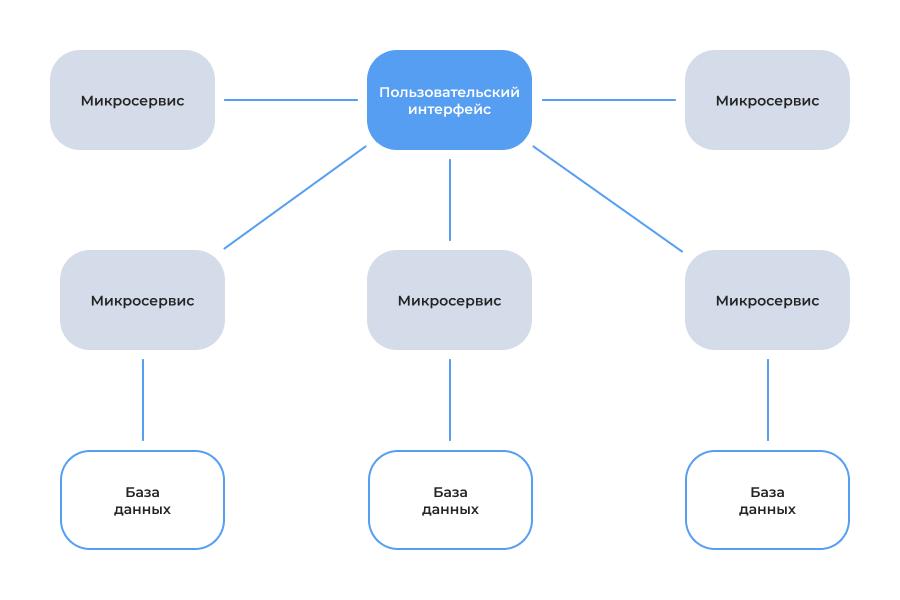
\includegraphics[width=0.9\hsize]{fig/microservices.png}\\[2mm]
\caption{Микросервисная архитектура}\label{fig:microservices}
\end{center}
\end{figure}

Преимущества микросервисной архитектуры:

\begin{enumerate} 
  \item слабая связанность — благодаря высокой степени изоляции, сбой в одном сервисе не затронет систему в целом;
  
  \item высокая степень масштабируемости — каждый сервис может разрабатываться, внедряться и масштабироваться по отдельности;
  
  \item разделение кодовых баз — каждый сервис имеет отдельную кодовую базу и может быть разработан с использованием разных языков программирования.
\end{enumerate}

Недостатки микросервисной архитектуры:

\begin{enumerate} 
  \item высокие требования к скорости канала между сервисами;
  
  \item сложность реализации взаимодействия между сервисами и их комплексном тестировании.
\end{enumerate}

Для реализации информационной системы «Личный кабинет абитуриента» выбрана микросервисная архитектура, благодаря которой, разработка клиентской и серверной части может вестись параллельно, а функционал информационной системы может быть легко расширен путем подключения новых сервисов.

На текущий момент, реализовано одностраничное веб-приложение, сервис REST-API для личного кабинет абитуриента, база данных, хранящая данные личного кабинета абитуриента, сервис обновления справочников, интеграция с системой учета «1С Университет», сервис резервного копирования, файловая система, сервис REST-API ФИАС, база данных, хранящая сведения об адресах, сервис обновления данных ФИАС. Общую конфигурацию и топологию информационной системы можно увидеть на диаграмме развертывания (рисунок \ref{fig:diagramdeploy}).

\begin{figure}[H]
\begin{center}
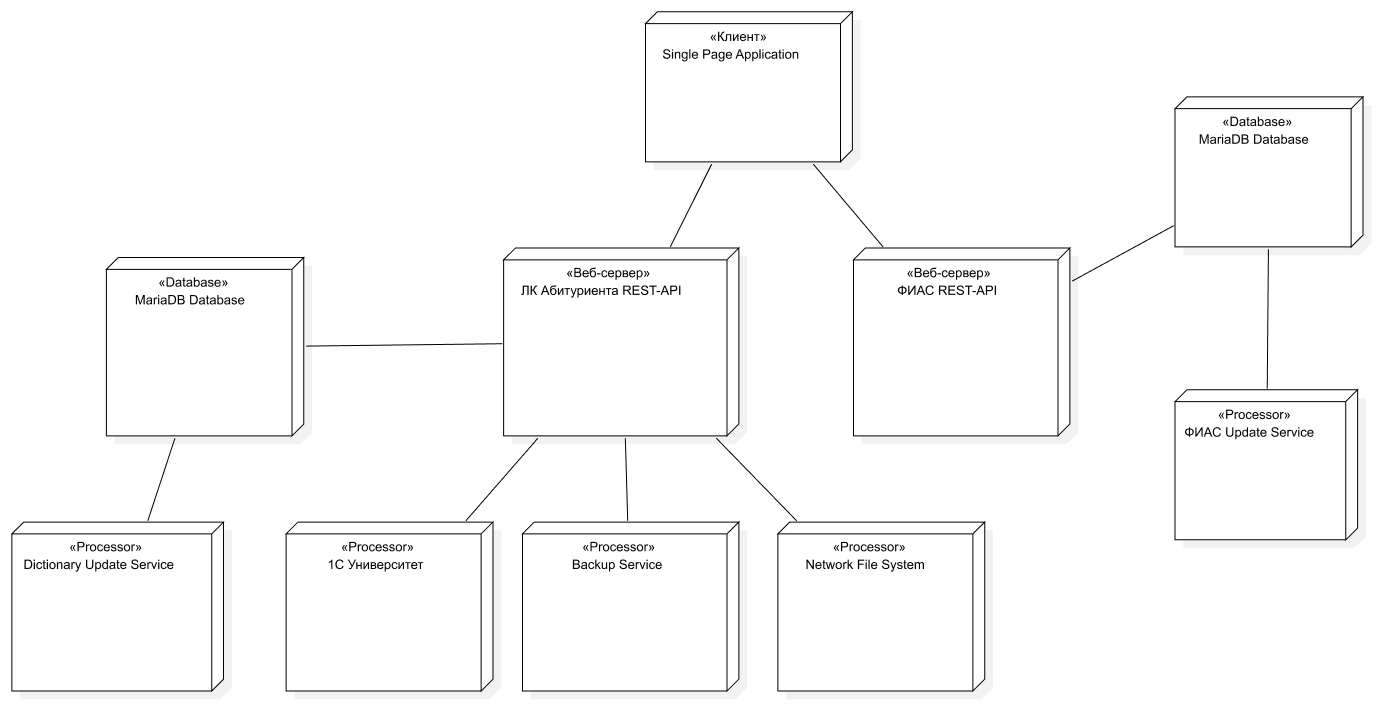
\includegraphics[width=1\hsize]{fig/diagram-deploy.png}\\[2mm]
\caption{Диаграмма развертывания информационной системы «Личный кабинет абитуриента»}\label{fig:diagramdeploy}
\end{center}
\end{figure}

Клиентская часть информационной системы будет реализована в виде одностраничного приложения. Single page application (SPA) — одностраничное веб-приложение, загружающие одну HTML-страницу и благодаря динамическому обновлению с помощью AJAX запросов, загружает данные и дополнительные страницы. Данные подход позволяет реализовать гибкий и отзывчивый интерфейс, поскольку все необходимые ресурсы загружаются без перезагрузки веб-страницы \cite{spa}.

\section{Проектирование пользовательского интерфейса}

Перед началом реализации клиентской части информационной системы, необходимо спроектировать все основные шаблоны веб-приложения, а также те части веб-приложения, интерфейс которых требует предварительного согласования.

Шаблоном в одностраничных приложениях называется компонент, который содержит в себе некоторые повторяющиеся на разных страницах элементы, а также основную часть, которая меняется на разных страницах \cite{designinfsystems}.

В веб-приложении «Личный кабинет абитуриента» будет использоваться два шаблона.

Шаблон для представлений авторизация (рисунок \ref{fig:templateauth}), регистрация (рисунок \ref{fig:templatereg}), восстановления пароля, будет содержать в себе шапку, место для основного содержимого страницы и подвал.

\begin{figure}[H]
\begin{center}
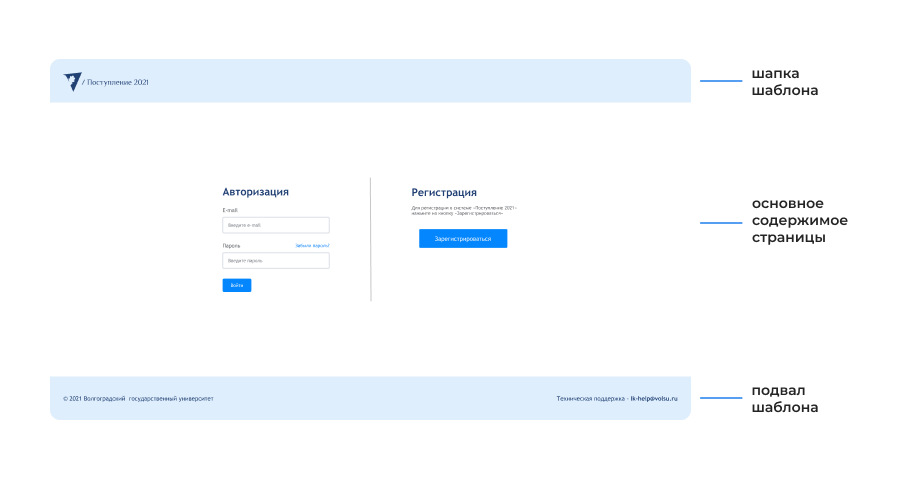
\includegraphics[width=1\hsize]{fig/template.png}\\[2mm]
\caption{Спроектированный шаблон для представления авторизация}\label{fig:templateauth}
\end{center}
\end{figure}


\begin{figure}[H]
\begin{center}
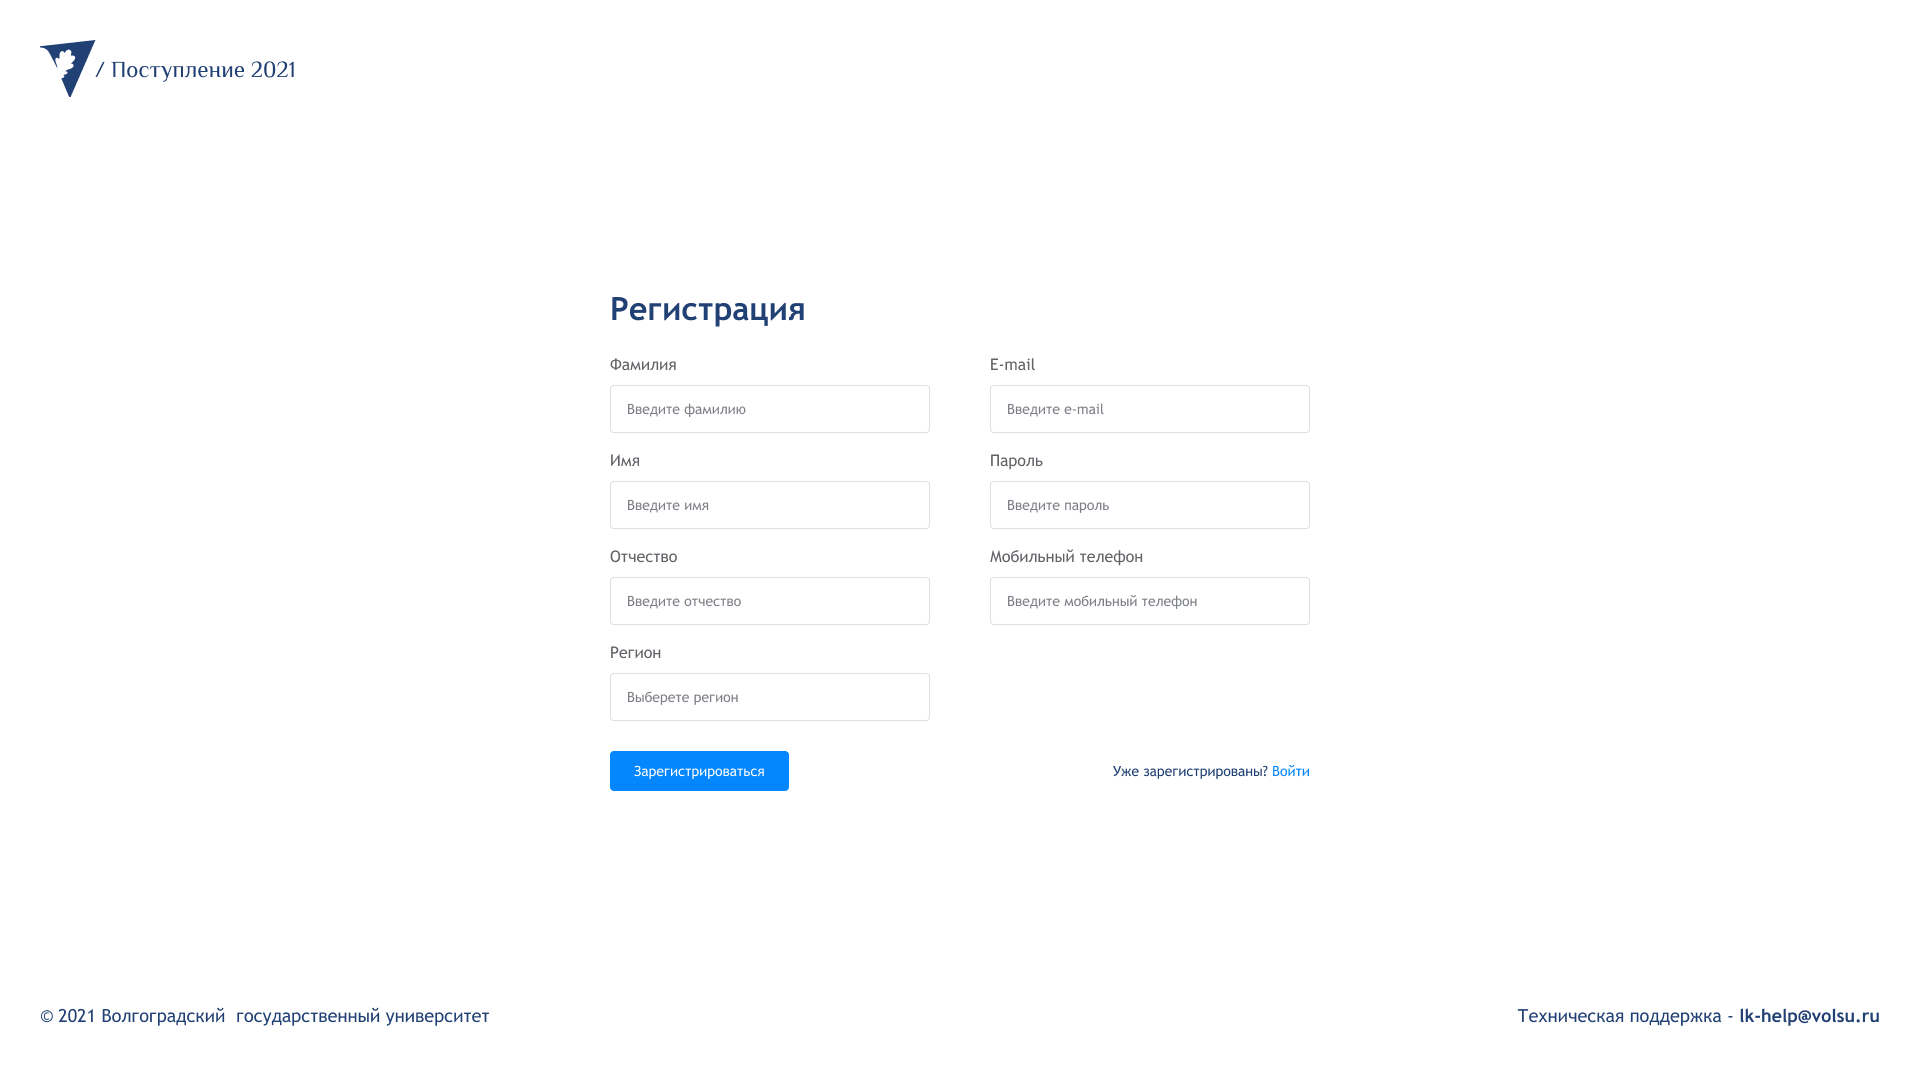
\includegraphics[width=1\hsize]{fig/template-reg.png}\\[2mm]
\caption{Спроектированный шаблон для представления регистрация}\label{fig:templatereg}
\end{center}
\end{figure}

Основной шаблон, используемый для внутренних страниц личного кабинета, содержит в себе навигационное меню и часть для основного содержимого страницы (рисунок \ref{fig:templatemain}).

\begin{figure}[H]
\begin{center}
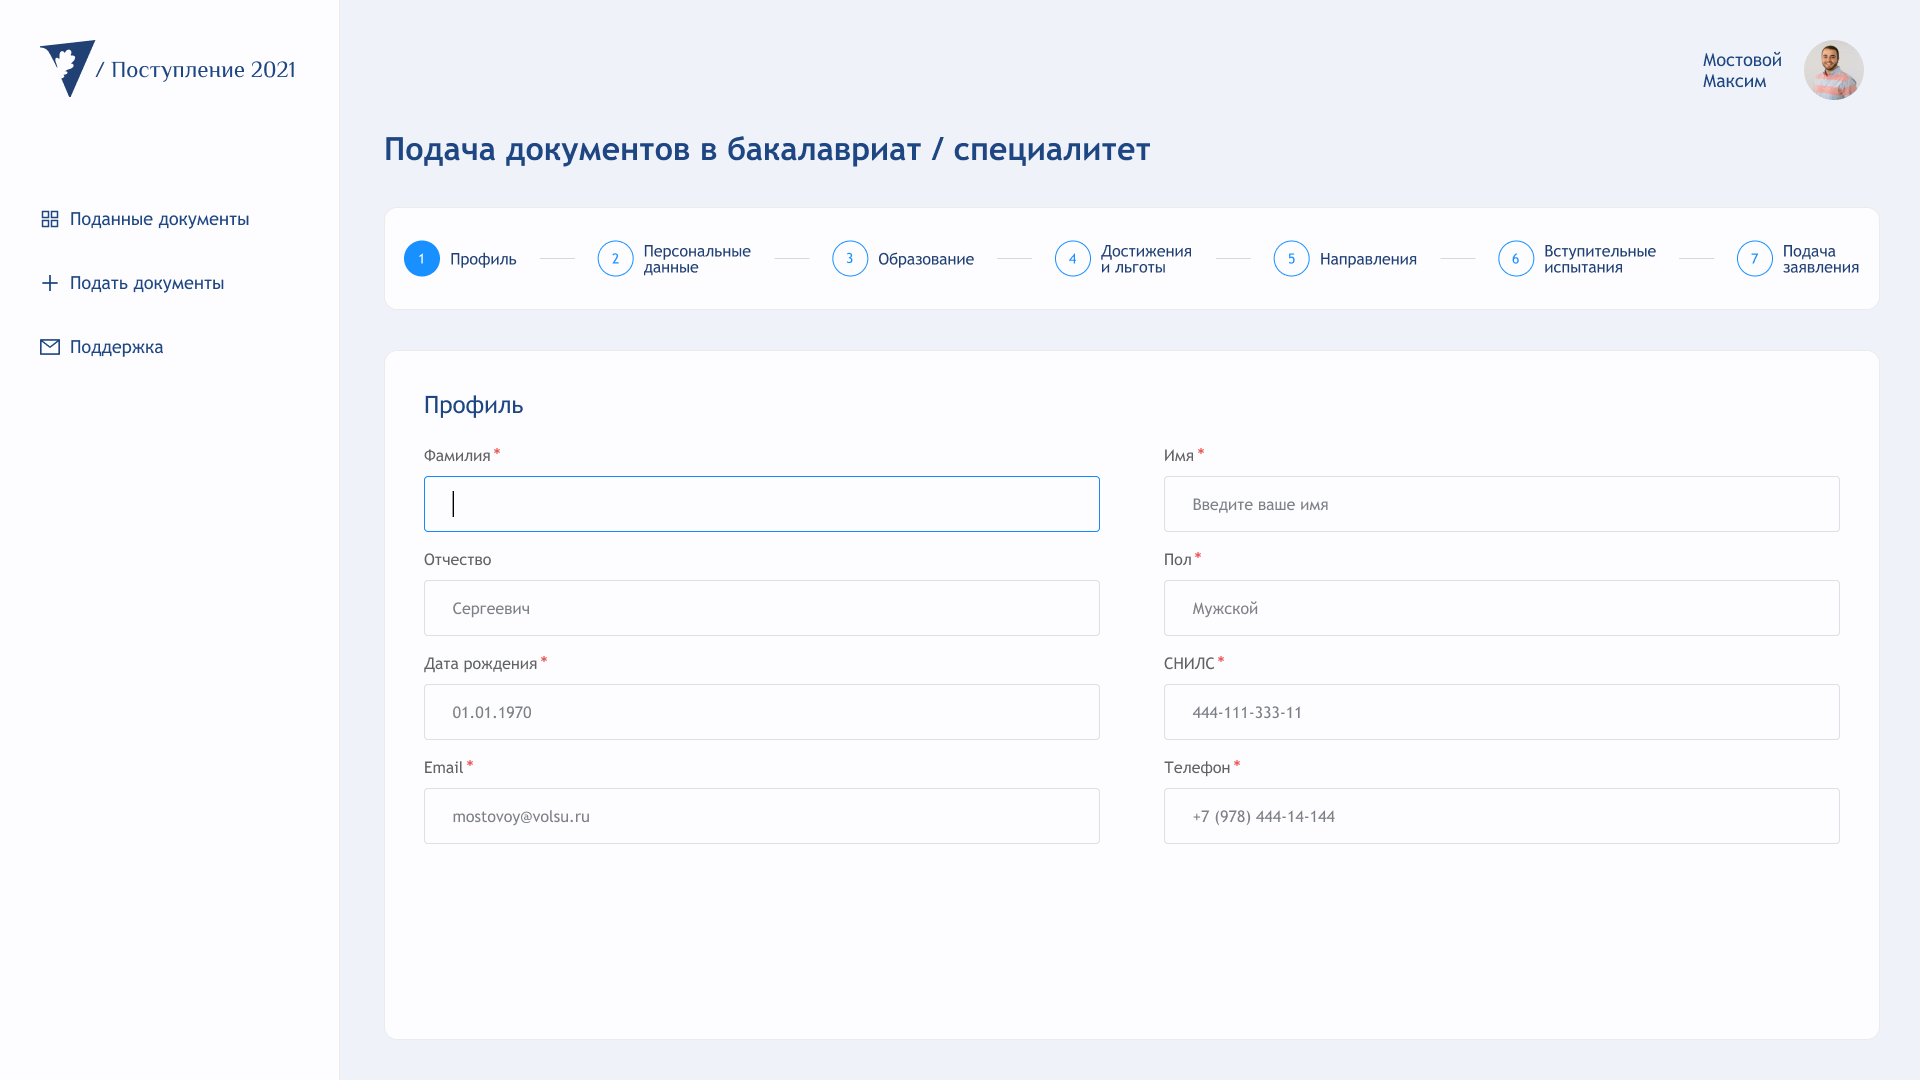
\includegraphics[width=1\hsize]{fig/main-layout-design.png}\\[2mm]
\caption{Спроектированный шаблон для внутренних страниц личного кабинета}\label{fig:templatemain}
\end{center}
\end{figure}

\chapter{Оформление библиографии}\label{Bib_chapter}

Для оформления списка литературы в шабоне используется система Bib\LaTeX.
Программное обеспечение для создания форматированных списков библиографии
Bib\LaTeX, позволяет упростить и (полу)автоматизировать процесс оформления
списка литературы. 

Для использования Bib\LaTeX{} необходимо записать список источников, на которые
вы ссылаетесь в своем тексте, в специальный файл с расширением .bib (Bib.bib).
Bib\LaTeX{} файл состоит из записей, которые начинаются с символа \verb|@| и
указанием типа записи. Что бы ни было записано в вашем bib-файле,
Bib\LaTeX{} по умолчанию включает в список литературы только те источники, на
которые вы ссылаетесь с помощью команды \verb|\cite|. Использовать команду
\verb|\nocite| для включения записей, на которые нет ссылок в тексте,
запрещается. Пример библиографической записи~\cite{Jackson2021TheOO}
в bib-файле приведен в листинге~\ref{ls:02}.

\begin{lstlisting}[caption={Пример библиографической записи}, label={ls:02}, language=TeX]
@article{Jackson2021TheOO,
  title={The origin of low-surface-brightness galaxies in the 
  dwarf regime},
  Ryan A. Jackson and Garreth Martin and Sugata Kaviraj 
  and Marius Ramsoy and Julien Devriendt and Thomas M. Sedgwick 
  and C. Laigle and H. Choi and Ricarda S Beckmann and Marta 
  Volonteri and Yohan Dubois and Christophe Pichon 
  and  Sukyoung K. Yi and Adrianne D. Slyz and Katarina Kraljic 
  and Taysun Kimm and S{\'e}bastien Peirani and Ivan K Baldry},
  journal={Monthly Notices of the Royal Astronomical Society},
  year={2021},
  volume={502},
  pages={4262--4276}
}
\end{lstlisting}

В первой строке, сразу после \verb|@article{|, стоит уникальная библиографическая
метка \verb|Jackson2021TheOO|; при ссылках в тексте на указанную работу
необходимо написать  \verb|\cite{Jackson2021TheOO}|. Далее идут поля записи,
также разделенные запятыми  Смысл большинства полей ясен из их названия. 

Для заполнения \verb|bib|-файла можно воспользоваться библиографическими базами
данных, которые позволяют выгрузить готовую запись в \verb|bib|-файл. Пример
такой базы и экспорта цитирований приведен на рисунке~\ref{fig:BibTex} 

\begin{figure}[h!]
\begin{center}
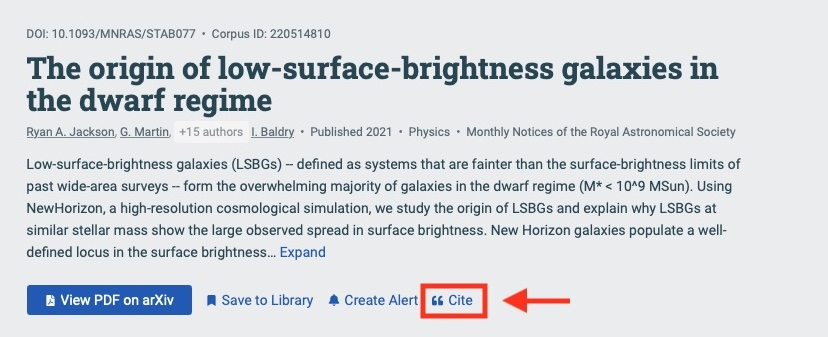
\includegraphics[width=0.8\hsize]{bib-1.jpg}\\[2mm]
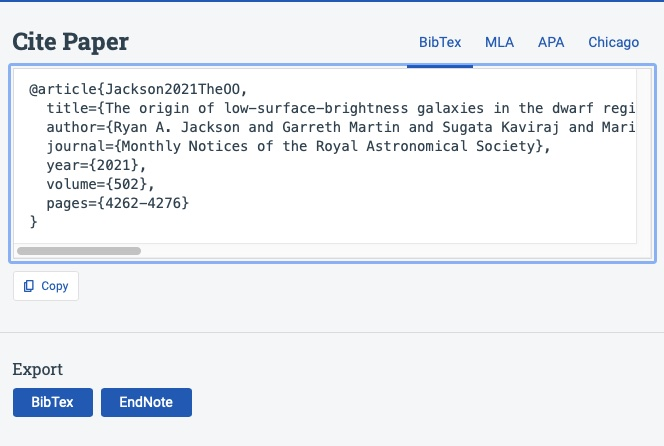
\includegraphics[width=0.8\hsize]{bib-2.jpg}\\[2mm]
\caption{Пример экспорта Bib\TeX-файла на примере системы SemanticScholar}\label{fig:BibTex}
\end{center}
\end{figure}

\newpage
\textbf{ВНИМАНИЕ!}

К списку источников предьявляютя особые требования. Это касается как его
содержания, так и количества источников, на которые вы ссылаетесь в своем
отчете. В первой строке таблицы~\ref{tab:lit} указан номер курса, для
которого в строке ниже приведено минимальное общее количество источников,
на которые есть ссылки в работе. В последующих строках приведено минимальное
количество источников разных типов. Под научно-периодической литературой
подразумевается наличие ссылок на статьи в периодических тематических журналах.

\begin{table}[h]
\caption{Название таблицы. Таблицы следует размещать в основном тексте рядом с первым цитированием.}
\label{tab:lit}
\begin{center}
\begin{tabular}{|p{7.5 cm}|c|c|c|c|c|}
\hline
 Номер курса & 2 & 3 & 4 & 5 & 6\\
\hline
Общее количество используемой литературы из них: & > 15 & > 20 & > 25 & > 30 & > 30 \\
\hline
- на иностранных языках & $\ge$4 & $\ge$5 & $\ge$6 & $\ge$7 & $\ge$7 \\
\hline
- текущая научно-периодическая литература (после 2010 г.)& $\ge$3 & $\ge$5 & $\ge$7 & $\ge$7 & $\ge$7  \\
\hline
- литература 21 века & $\ge$10 & $\ge$15 & $\ge$21 & $\ge$21 & $\ge$21 \\
\hline
\end{tabular}
\end{center}
\end{table}

\conclusion
Основной целью данной работы являлось проектирование и описание функциональных возможностей программного обеспечения для статического анализа кода системы компьютерной верстки TeX, выдающей в качестве результата информационные сообщения, которые помогут исправить моменты несоответствия оформления работы относительно проверяемого конфигурационного файла. Для достижения цели были выполнены следующие задачи:
    \begin{enumerate}    
    \item выявление анализируемых характеристик;    
    \item создание и описание модели конфигурационного файла.
    \item описание алгоритма выполняемых функций проверки характеристик!   
    \item Cоставление хода работы программы;
    \end{enumerate}

В ходе данной работы были изучены материалы, связанные со статическим анализом, включая цели, задачи, преимущества и недостатки, была рассмотрена концепция написания документов с помощью системы верстки \TeX, было осуществлено ознакомление с основными командами \LaTeX, их аргументами и опциями. 

Изученная теория применена на практике, а именно – создан и описан конфигурационный файл являющийся шаблоном, по которому необходимо выполнять статический анализ, а так же описаны механизмы его проведения. А так же выполнено описание хода работы и алгоритмов функций програмного обеспечения.

По итогам работы был сфомированн отчет в системе \LaTeX.
В результате выполнения работы были сформированы следующие компетенции: 

При выполнении работы был проведен поиск нужной информации по теме «Разработка программного обеспечения для статического анализа кода системы компьютерной верстки TeX» и ее анализ,  что соответствует компетенции: 

УК-1. Способен осуществлять поиск, критический анализ и синтез информации, применять системный подход для решения поставленных задач.

Была проделана работа генерации идеи и постановки задачи, а также
выбор технологий с научным руководителем, что соответствует компетенции:

УК-4. Способен осуществлять деловую коммуникацию в устной и письменной формах на государственном языке Российской Федерации и иностранном(ых) языке(ах).

Были оценены и проанализированы требования к исходным данным и программе статичего анализа системы верстки \TeX\verb| |и выбраны подходящие технологии для ее реализации, что соответствует компетенции:

ПК-5. Способен анализировать требования к программному обеспечению и разрабатывать технические спецификации на программные компоненты.

Был разработан и описан проект программы для статического анализа системы верстки \TeX, что соответствует компетенции:

ПК-6. Способен проводить концептуальное, функциональное и логическое проектирование информационных систем.

Были заложены основны и требования к пользовательскому интерфейсу, а также подобраны технологии, для его реализации, что соответствует компетенции:

ПК-7. Способен проектировать пользовательские интерфейсы по готовому образцу или концепции интерфейса.

\printbibliography[heading=bibintoc]
\end{document}